
%%%%%%%%%%%%%%%%%%%%%%%%%%%%%%%%%%%%%%%%%%%%%%%%%%%%
%    Jordan Scott    %
%%%%%%%%%%%%%%%%%%%%%%%%%%%%%%%%%%%%%%%%%%%%%%%%%%%%
%\documentclass{article}

%\usepackage[utf8]{inputenc}
%\usepackage[english]{babel}
%\usepackage{graphicx}


%\begin{document}
	
	%\title{CS6000 Journal}
	%\author{Jordan Scott} 
	%\maketitle
	
	\section{\textbf{CS6000 Journal - Jordan Scott}}
	
	
	\begin{figure}
		\centering
		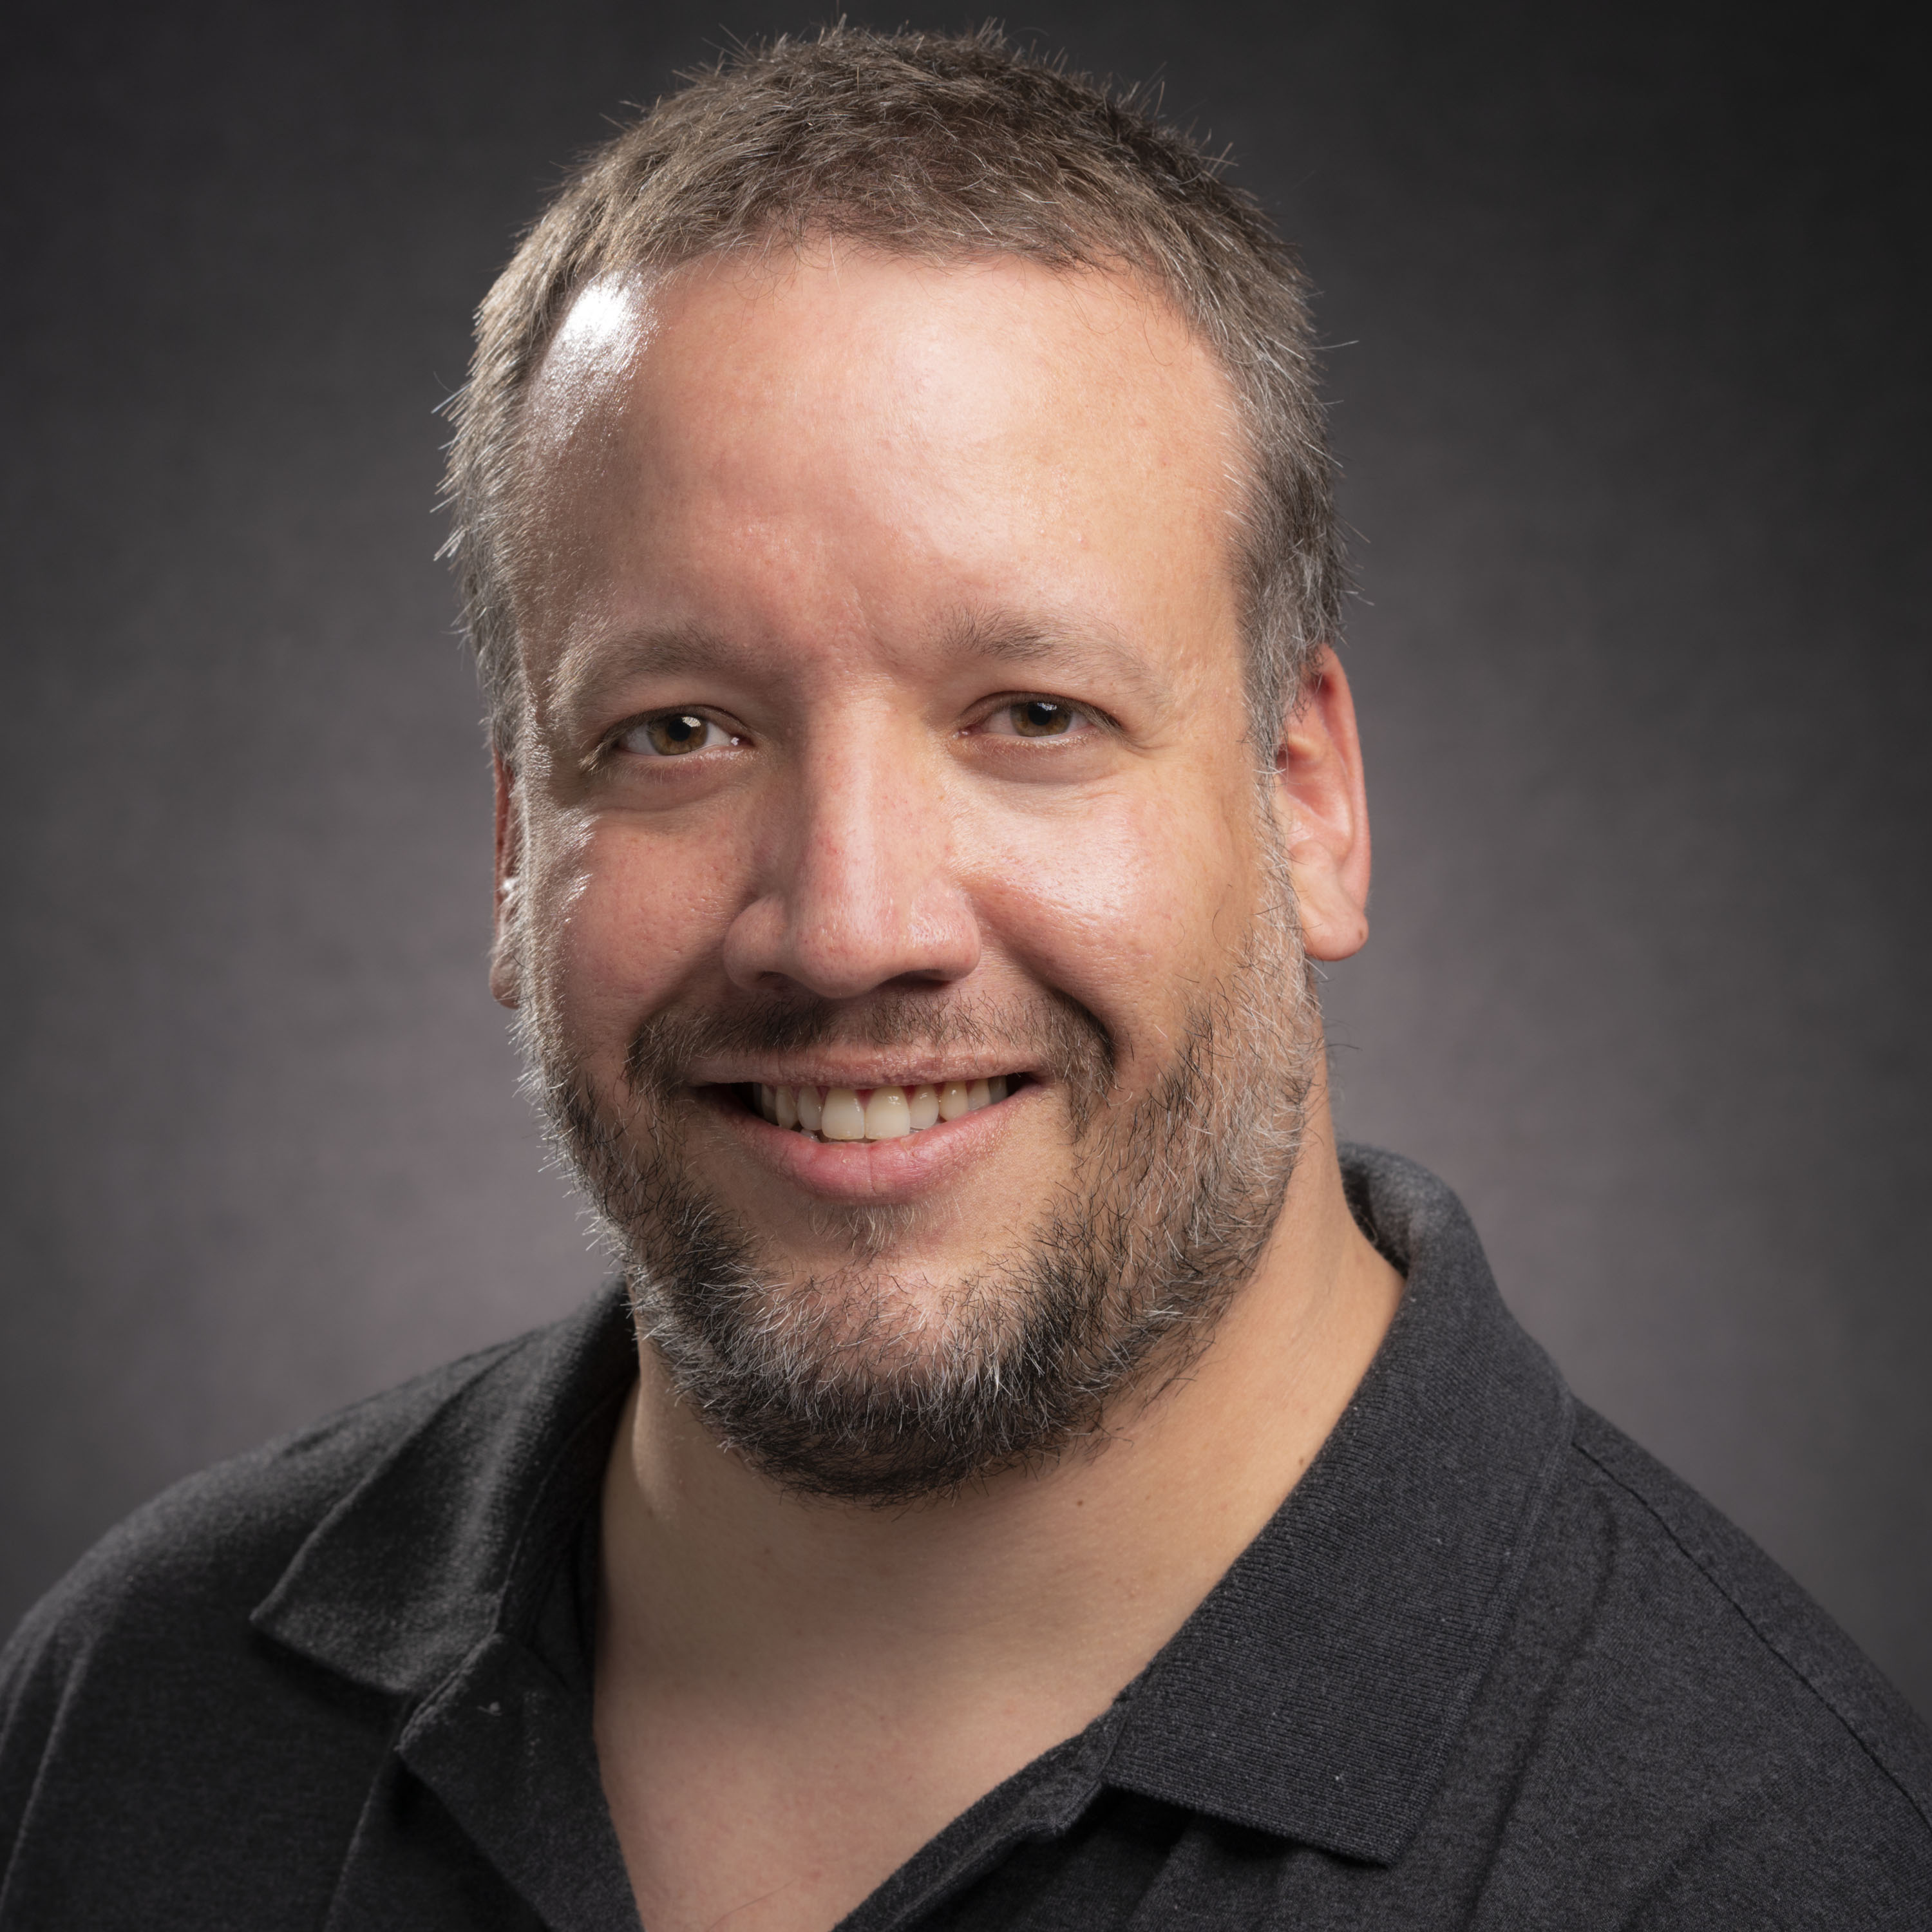
\includegraphics[width=0.4\linewidth]{jordan.jpg}
		\caption{Jordan Scott}
	\end{figure}

	\paragraph*{Contact Info: } jscott21@uccs.edu \\
	https://www.linkedin.com/in/jordan-cancer-scott/\\
	https://github.com/jordanmscott/uccs


	\paragraph*{About Me}
		
		
		
	I am just starting my PhD in Security program. My goal for this course is to get into a research frame of mind, learn the modern tricks and tips, and help refine my dissertation topic.
	
	
	I am really interested in learning more about zotero and latex. I gained some experience with zotero last year, but previously I've only been aware of manual tracking and editing. It's nice to know that technology has evolved quite a bit with research and data management.
	

	I have done stand-up comedy twice. My set was mostly cybersecurity related and I received a number of laughs. I'm not sure if my comedy career will continue, but my career will definitely be full of comedy. 
	

	
	
	
	\paragraph*{\textbf{Questions}}
	
	Question and Answers
	
	
	Question 1 - Hi Jordan, I am just beginning my PhD program this year also!  I am learning a lot, trying to wrap my head around many things.  Dr. Kalita is my faculty advisor and I am studying AI.  I don't have a definite plan of study yet.  I'm learning so many things from this class about research. Another learning curve.  I don't know about you, but I am spending endless hours figuring out LaTex and github. I'll get there, though.  What are your impressions so far?
	
	
	Answer 1 - I like how the research methodologies have used software best practices to advance. The learning curve definitely exists though. I think this class has done a great job in getting us on the same page and moving towards using the tools properly. I suspect it will be a huge help later down the line when we are in a hundred page documument with hundreds of references.

	
	Question 2 - Question for Jordan Scott from James Peng: Hi, Jordan, I would like to ask you what is the most challenging experience/ things when you are  in comedy industry? I always feel you guys are awesome, like "positive/ joy-sharing version of lawyers", very good at public speaking, rhetoric, and know very well with the "jury".
	
	
	Answer 2 - Comedy is some awkward balance of saying what is on your mind, taking risk regardless of opinions, timing, and getting people into a mood. I think it probably has some of the same science behind it as music. Instead of beats per minute, its laughs per joke. My biggest challenge is memory though. I have a hard time remembering a script so I do more reading than natural delivery like the pros. I can talk and just keep going without a script, but the timing and order of things matter enough to where scripts have advantages. I think that's something I will just have to keep working on.


	\paragraph*{\textbf{Merge Conflict Notes:}}
	
	
	Not having access to the project seemed frustrating and took a bit to even figure out that was the problem. For my setup, I chose to use TeXstudio on a virtual box. The git clone part was easy. Getting the Assignment3 file to build was not. There were dependencies I needed to download/install into TeXstudio which was a challenge in itself, all related to the csvsimple function. Eventually got all that working. Then trying to figure out git itself... Got the commit part, the pull, the merge (had to install and configure a compare tool), and then the push. It's all working now and I definitely have a better understanding of git. The branches and stuff will get more interesting too. Anyways, I think I'm ready to start developing reports using this IDE/Git setup instead of manually transfering from overleaf.
		
	
%\end{document}

<<<<<<< HEAD
 
=======
\textbf{Question from Maximus to Jordan}: Hi Jordan, glad you can make jokes from a topic such as cybersecrity. One of the surprising things I discovered in these discussions, as I am reading through the comments, is we have people with really different backgrounds and interests in this field and they are mostly competent. How do you think your passion for comedy would contribute to research in a logical field like cybersecurity?
>>>>>>> 395e345b13e2f4e534ee67e0916c1dac96bbad64
